\documentclass[aspectratio=169,11pt]{beamer}

\usepackage{booktabs}
\usepackage{array}
\usepackage{graphicx}
\usepackage{siunitx}
\usepackage{xurl}
\usepackage{xcolor}

\usetheme{Madrid}
\usecolortheme{default}
\setbeamertemplate{navigation symbols}{}
\setbeamertemplate{footline}[frame number]
\graphicspath{{images/neural_network_fit_results/}}

\newcommand{\goodtext}[1]{\textcolor{green!45!black}{#1}}
\newcommand{\warntext}[1]{\textcolor{red!65!black}{#1}}
\newcommand{\notetext}[1]{\textcolor{blue!65!black}{#1}}
\newcommand{\pathtext}[1]{\texttt{\footnotesize\detokenize{#1}}}
\newcolumntype{L}[1]{>{\raggedright\arraybackslash}p{#1}}
\newcolumntype{R}[1]{>{\raggedleft\arraybackslash}p{#1}}

\title[NN Fitting Results]{Neural Network Fitting Results}
\subtitle{Inference evaluation of the MLP penetration surrogate on the clean split}
\author{Linan Jiang}
\institute{Aalto University}
\date{15 April 2026}

\begin{document}

\begin{frame}
  \titlepage
\end{frame}

\begin{frame}{Evaluation Target}
\small
\begin{block}{Source of this result set}
The inference script loads the weights from the refined student model and predicts the penetration mean and predictive standard deviation point by point on the \texttt{series\_wide\_clean} trajectories.
\end{block}

\vspace{0.4em}
\begin{tabular}{L{0.30\linewidth}L{0.60\linewidth}}
\toprule
Item & Setting \\
\midrule
Refinement run & \pathtext{distill_cdf_onset_v2_20260410_103413} \\
Teacher run & \pathtext{stage2_engineered_nll_a_only_20260410_020607} \\
Evaluation split & \texttt{clean}, time window \SIrange{0}{5}{ms} \\
Input features & time, tilt angle, plume count, injection duration, control backpressure \\
Outputs & predicted penetration \(\mu\), predicted uncertainty \(\sigma\), onset logit \\
\bottomrule
\end{tabular}

\vspace{0.6em}
\footnotesize
Raw result folder: \pathtext{MLP/inference_testing/rmse_eval_clean_20260415_092112}
\end{frame}

\begin{frame}{Data Scale and Overall Error}
\small
\begin{columns}[T,onlytextwidth]
\begin{column}{0.48\linewidth}
\begin{tabular}{L{0.55\linewidth}R{0.32\linewidth}}
\toprule
Metric & Value \\
\midrule
CSV files & 266 \\
Trajectories & 14,972 \\
Prediction points & 399,738 \\
Truth range & \SIrange{0.00}{95.88}{mm} \\
\midrule
RMSE & \SI{6.90}{mm} \\
MAE & \SI{5.16}{mm} \\
Bias & \SI{-1.29}{mm} \\
Median absolute error & \SI{3.97}{mm} \\
P90 / P95 absolute error & \SI{11.20}{mm} / \SI{14.17}{mm} \\
Range-normalized RMSE & 7.19\% \\
\bottomrule
\end{tabular}
\end{column}

\begin{column}{0.48\linewidth}
\begin{block}{How to read the metrics}
\footnotesize
\begin{itemize}
  \item \goodtext{Typical error is modest}: the median absolute error is about \SI{4}{mm}.
  \item \notetext{The global bias is negative}: on average, the model under-predicts penetration by about \SI{1.3}{mm}.
  \item \warntext{Tail errors remain visible}: the P95 absolute error reaches \SI{14.2}{mm}; a subset of conditions or trajectories still drives the main risk.
\end{itemize}
\end{block}

\begin{block}{Uncertainty}
\footnotesize
\begin{itemize}
  \item Mean predicted \(\sigma\): \SI{6.36}{mm}
  \item 1\(\sigma\) coverage: 68.47\%
  \item 2\(\sigma\) coverage: 95.67\%
\end{itemize}
\end{block}
\end{column}
\end{columns}
\end{frame}

\begin{frame}{Predicted vs. Measured Penetration}
\begin{columns}[T,onlytextwidth]
\begin{column}{0.55\linewidth}
  \centering
  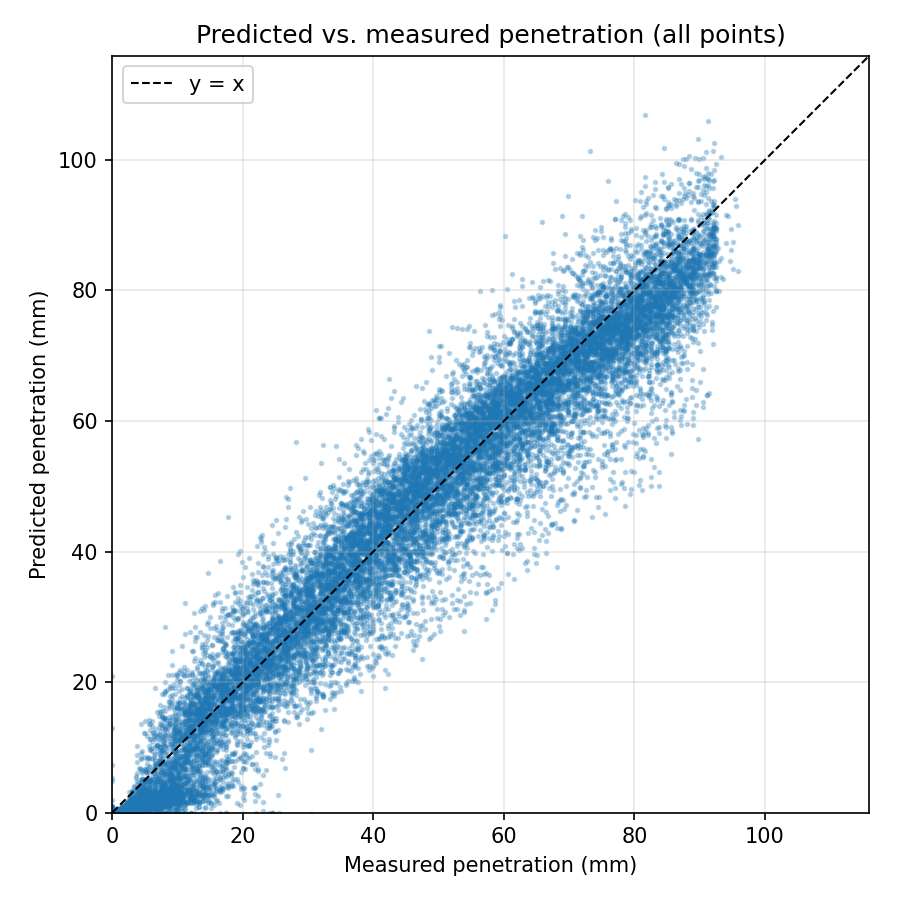
\includegraphics[width=\linewidth,height=0.73\textheight,keepaspectratio]{pred_vs_actual.png}
\end{column}
\begin{column}{0.41\linewidth}
\footnotesize
\begin{block}{Main observations}
\begin{itemize}
  \item Most points follow the \(y=x\) line, showing that the model captures the main penetration trend.
  \item Scatter increases in the high-penetration region, which is one of the main contributors to RMSE.
  \item A few nonzero predictions appear in the low-penetration region, reflecting timing and threshold uncertainty near onset.
\end{itemize}
\end{block}
\vspace{0.2em}
\footnotesize
Each point is one time sample. The axes are measured and predicted penetration.
\end{column}
\end{columns}
\end{frame}

\begin{frame}{Residual Distribution and Calibration}
\begin{columns}[T,onlytextwidth]
\begin{column}{0.56\linewidth}
  \centering
  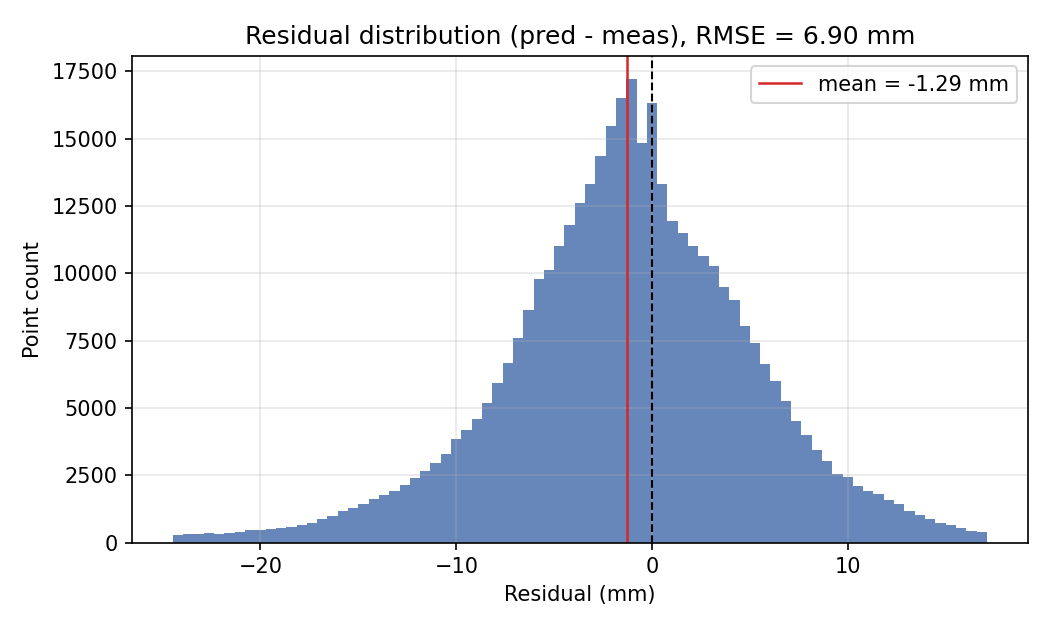
\includegraphics[width=\linewidth,height=0.72\textheight,keepaspectratio]{residual_histogram.png}
\end{column}
\begin{column}{0.40\linewidth}
\footnotesize
\begin{block}{Residual definition}
\[
e = \hat{y}_{\mathrm{pen}} - y_{\mathrm{pen}}
\]
\end{block}

\begin{itemize}
  \item Bias = \SI{-1.29}{mm}, so the model is slightly biased toward under-prediction.
  \item 1\(\sigma\) coverage = 68.47\%, close to the Gaussian one-sigma reference.
  \item 2\(\sigma\) coverage = 95.67\%, close to the Gaussian two-sigma reference.
  \item Predicted \(\sigma\) is usable at the global scale, but it cannot replace condition-by-condition error analysis.
\end{itemize}
\end{column}
\end{columns}
\end{frame}

\begin{frame}{RMSE Grouped by Experimental Folder}
\begin{columns}[T,onlytextwidth]
\begin{column}{0.57\linewidth}
  \centering
  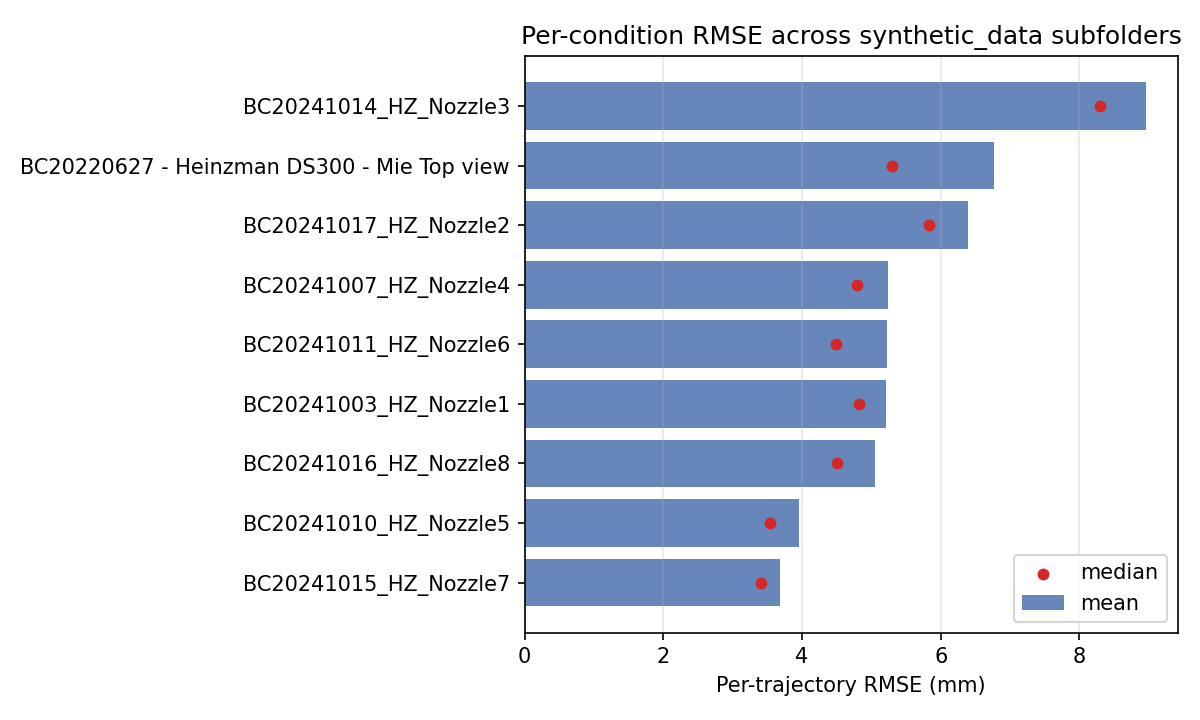
\includegraphics[width=\linewidth,height=0.68\textheight,keepaspectratio]{per_folder_rmse.png}
\end{column}
\begin{column}{0.39\linewidth}
\scriptsize
\begin{tabular}{L{0.62\linewidth}R{0.24\linewidth}}
\toprule
Folder & Mean RMSE \\
\midrule
Nozzle7 & \SI{3.68}{mm} \\
Nozzle5 & \SI{3.95}{mm} \\
Nozzle8 & \SI{5.05}{mm} \\
Nozzle1 & \SI{5.21}{mm} \\
Nozzle6 & \SI{5.22}{mm} \\
Nozzle4 & \SI{5.24}{mm} \\
Nozzle2 & \SI{6.40}{mm} \\
DS300 top view & \SI{6.77}{mm} \\
Nozzle3 & \SI{8.96}{mm} \\
\bottomrule
\end{tabular}

\vspace{0.3em}
\footnotesize
\begin{itemize}
  \item Best groups: Nozzle7 and Nozzle5, with RMSE below \SI{4}{mm}.
  \item Hardest group: Nozzle3, with mean RMSE near \SI{9}{mm}.
\end{itemize}
\end{column}
\end{columns}
\end{frame}

\begin{frame}{Well-Predicted Trajectory Group: Nozzle5 / T10}
\begin{columns}[T,onlytextwidth]
\begin{column}{0.62\linewidth}
  \centering
  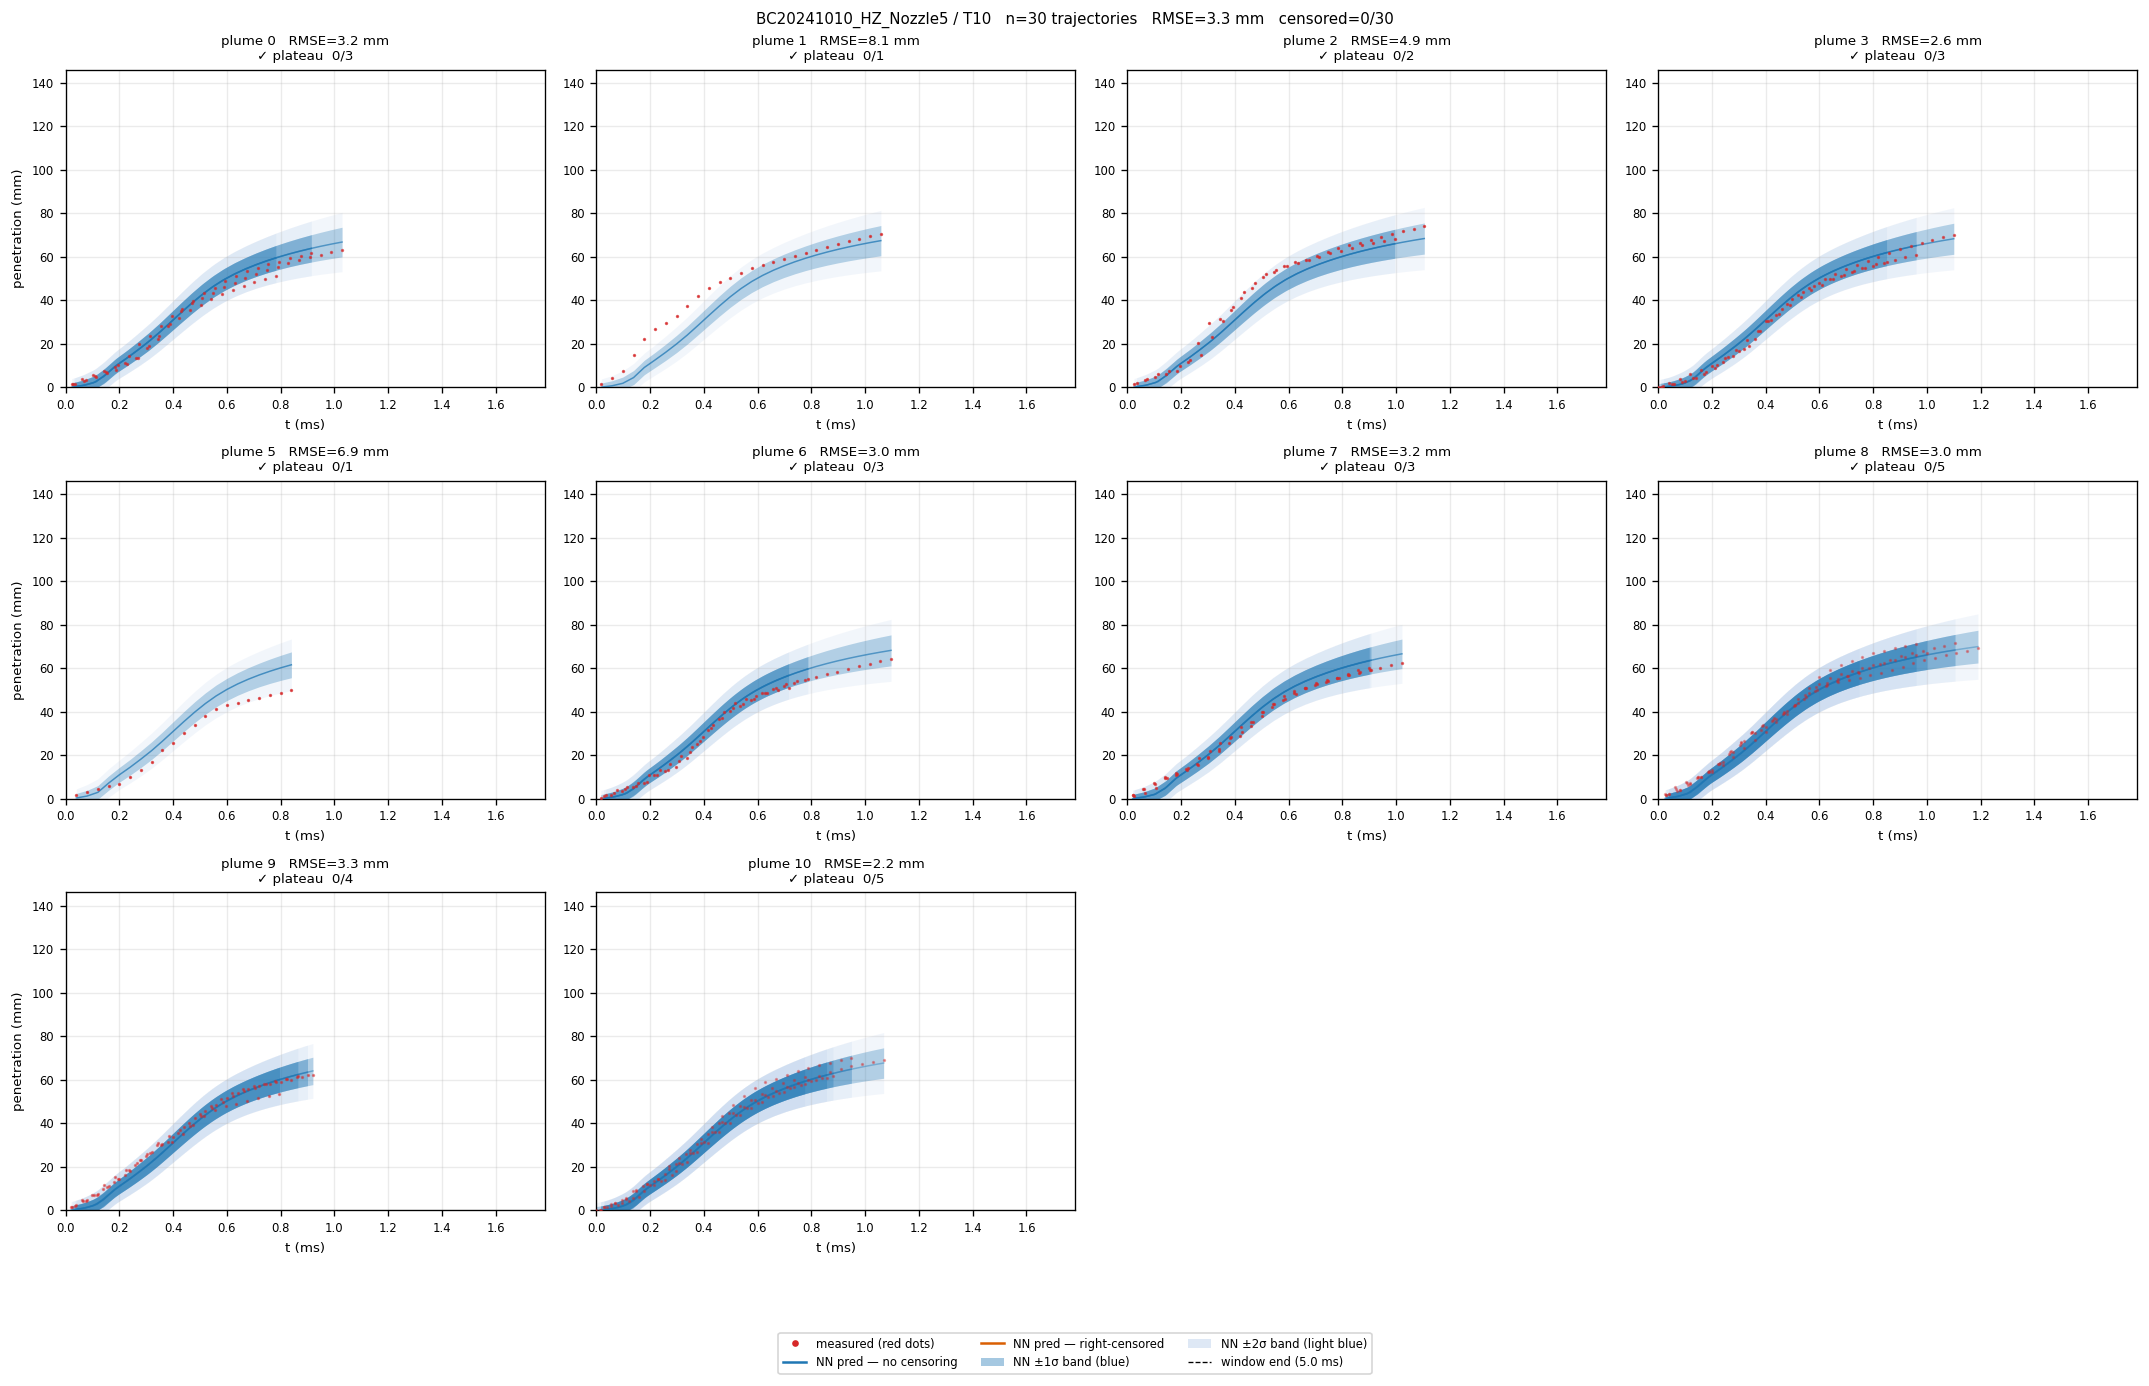
\includegraphics[width=\linewidth,height=0.62\textheight,keepaspectratio]{traj_nozzle5_T10.png}
\end{column}
\begin{column}{0.34\linewidth}
\footnotesize
\begin{block}{Representative characteristics}
\begin{itemize}
  \item Per-folder mean RMSE: \SI{3.95}{mm}
  \item 1\(\sigma\) coverage: 73.65\%
  \item 2\(\sigma\) coverage: 97.15\%
\end{itemize}
\end{block}

\begin{itemize}
  \item The growth trend is tracked consistently.
  \item The uncertainty band covers most plume/repeat trajectories.
  \item Engineered features and refinement capture the main condition dependence.
\end{itemize}
\end{column}
\end{columns}
\end{frame}

\begin{frame}{High-Error Trajectory Group: DS300 / T8}
\begin{columns}[T,onlytextwidth]
\begin{column}{0.62\linewidth}
  \centering
  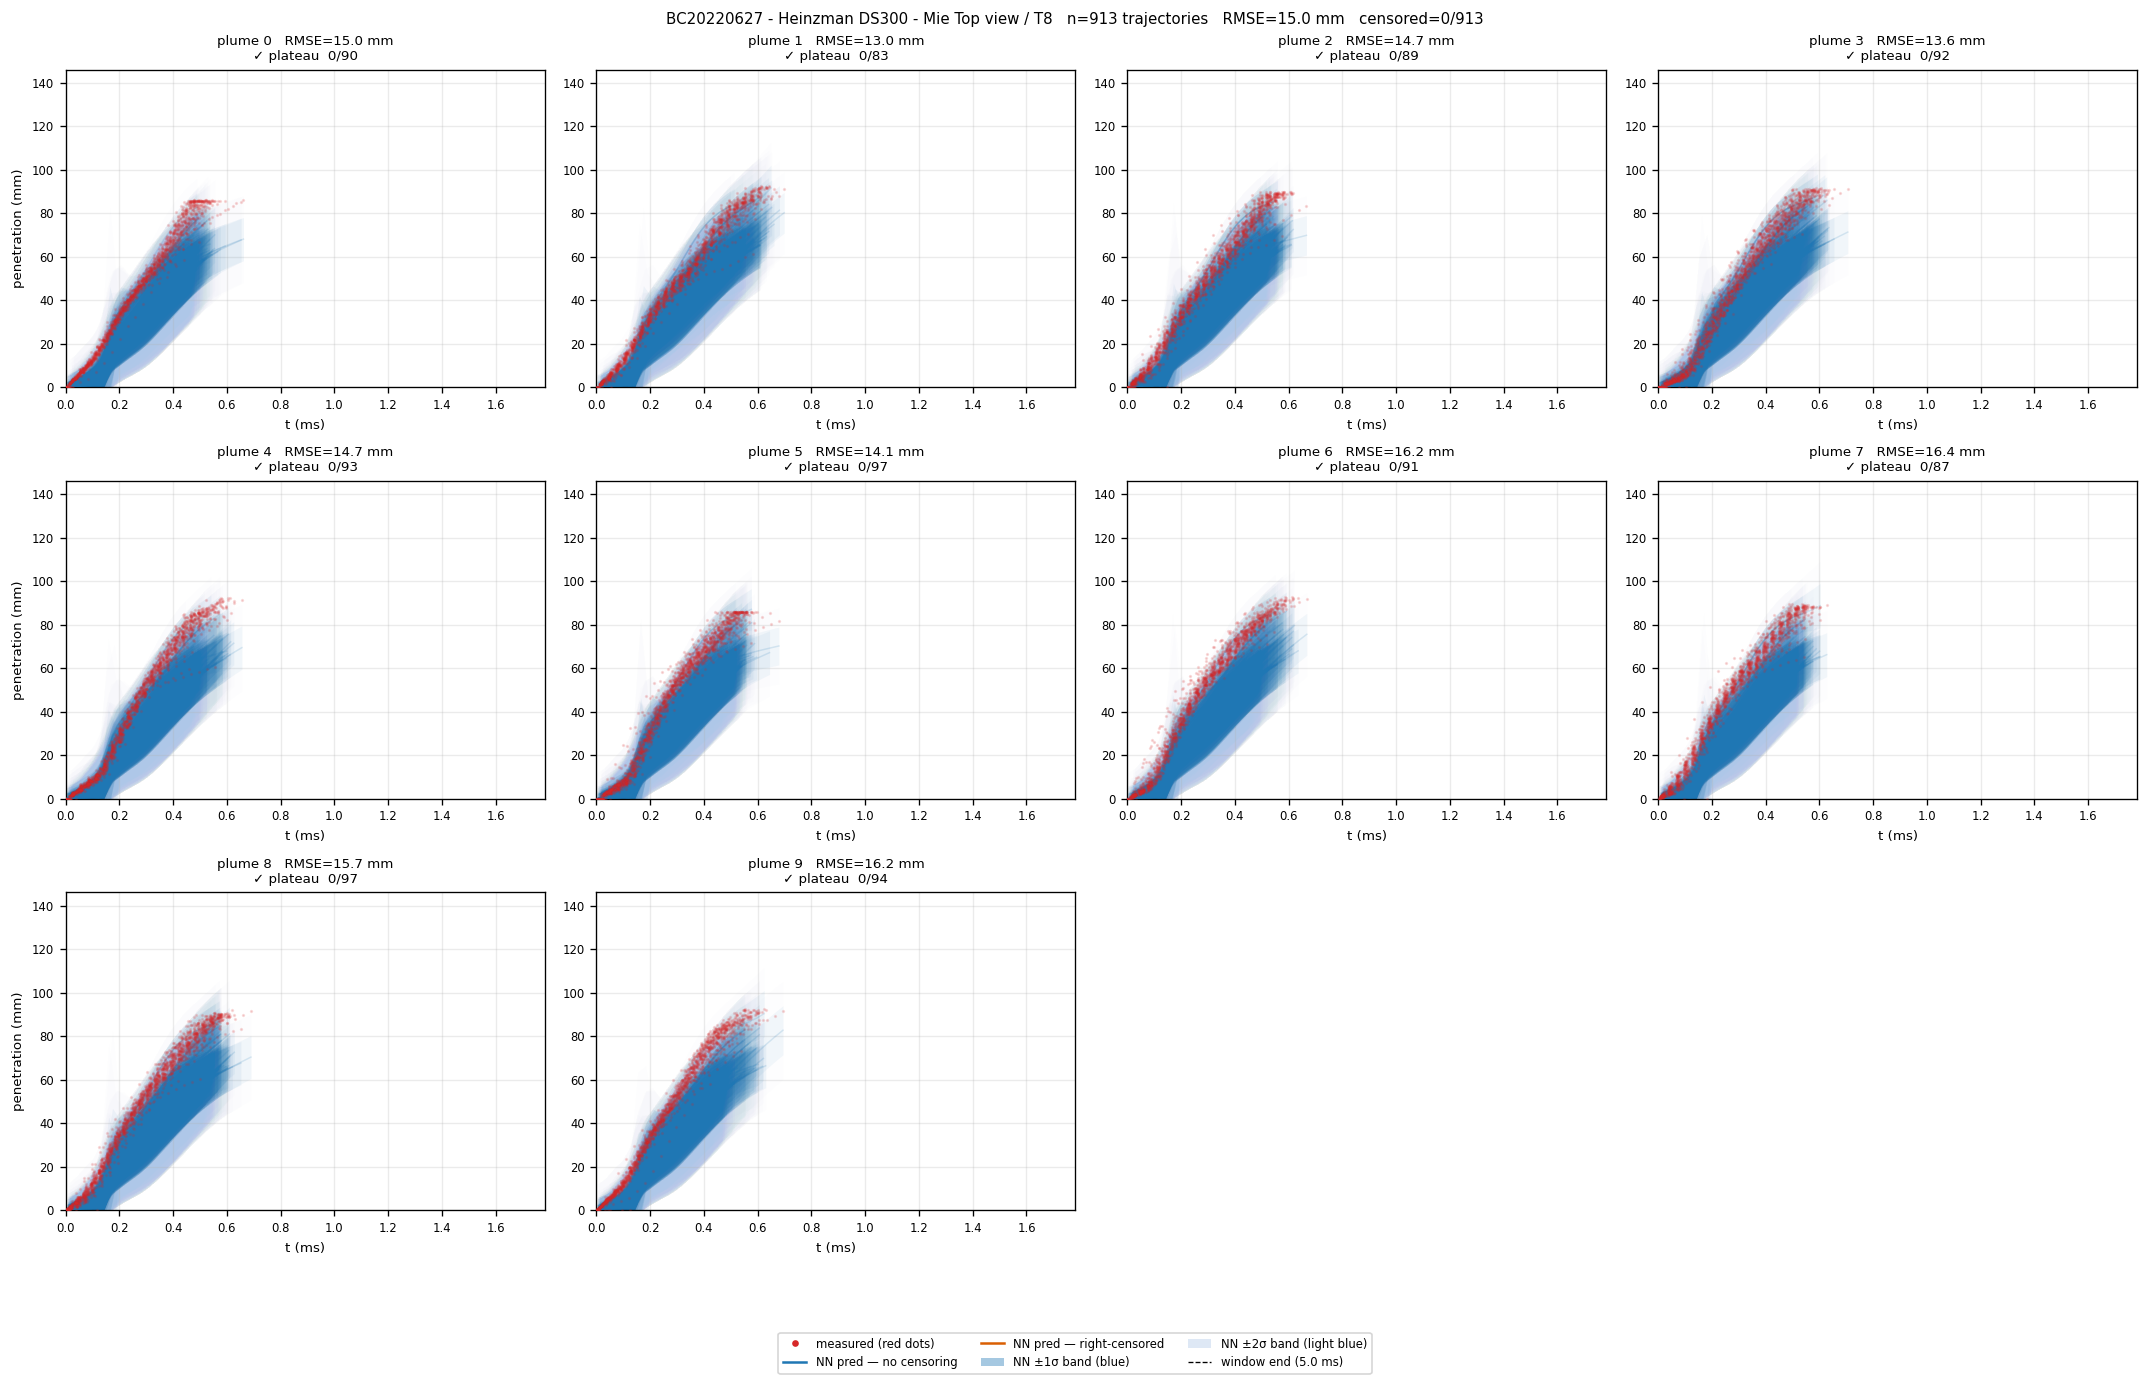
\includegraphics[width=\linewidth,height=0.62\textheight,keepaspectratio]{traj_ds300_T8.png}
\end{column}
\begin{column}{0.34\linewidth}
\footnotesize
\begin{block}{Risk signals}
\begin{itemize}
  \item DS300 folder mean RMSE: \SI{6.77}{mm}
  \item 1\(\sigma\) coverage: 60.00\%
  \item 2\(\sigma\) coverage: 92.98\%
\end{itemize}
\end{block}

\begin{itemize}
  \item Worst cases concentrate in DS300/T8, with RMSE around \SIrange{23.8}{24.5}{mm}.
  \item The low coverage indicates that uncertainty is still too narrow for outliers.
  \item Raw segmentation, delay alignment, and condition distribution should be checked.
\end{itemize}
\end{column}
\end{columns}
\end{frame}

\begin{frame}{Conclusions}
\small
\begin{enumerate}
  \item \goodtext{The overall fit is usable}: on the clean split, RMSE is \SI{6.90}{mm}, NRMSE is 7.19\%, and the median absolute error is \SI{3.97}{mm}.
  \item \goodtext{The uncertainty is reasonably calibrated overall}: 1\(\sigma\)/2\(\sigma\) coverage is 68.47\%/95.67\%, close to the Gaussian reference.
  \item \notetext{The error is not uniformly distributed}: Nozzle5/7 perform well, while Nozzle3, DS300, and some high-penetration trajectories contribute most of the tail error.
  \item \warntext{Next priorities}: perform segmentation QA, delay-alignment QA, and feature-coverage checks for high-error folders/tests, and evaluate whether folder-aware calibration is needed.
\end{enumerate}

\vspace{0.8em}
\begin{block}{Short thesis-ready conclusion}
The neural surrogate reproduces most penetration trajectories within the \SIrange{0}{5}{ms} window and provides predictive uncertainty that is reasonable at the global scale. Further improvement should focus on cross-dataset domain shift and a small number of high-error trajectories.
\end{block}
\end{frame}

\begin{frame}{File Index}
\small
\begin{tabular}{L{0.28\linewidth}L{0.60\linewidth}}
\toprule
Content & File \\
\midrule
Slides source & \pathtext{Thesis/neural_network_fit_results_slides_en.tex} \\
Compiled PDF & \pathtext{Thesis/neural_network_fit_results_slides_en.pdf} \\
Copied figures & \pathtext{Thesis/images/neural_network_fit_results/} \\
Result folder & \pathtext{rmse_eval_clean_20260415_092112} \\
Overall metrics & \pathtext{metrics_summary.json} \\
Per-folder table & \pathtext{per_folder.csv} \\
Per-trajectory table & \pathtext{per_trajectory.csv} \\
\bottomrule
\end{tabular}
\end{frame}

\end{document}
